\section{Method Supplements}
\begin{figure}[t]
\centering
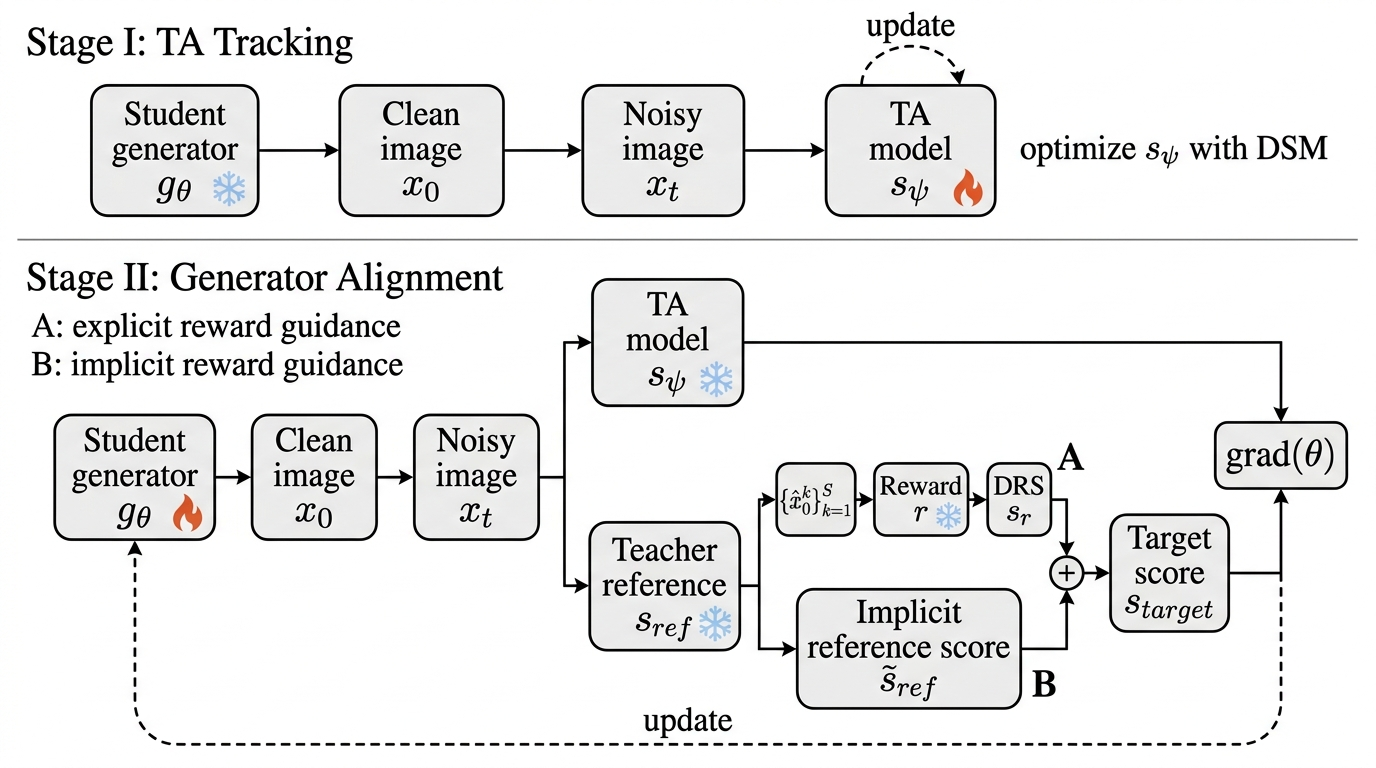
\includegraphics[width=0.95\linewidth]{pictures/Pipeline.png}
\caption{\textbf{The \textsc{Didr} training framework.} \textbf{Stage I (TA):} $s_\psi$ tracks the generator marginals via DSM. \textbf{Stage II (Generator):} $g_\theta$ is updated toward the reward-tilted target score $\tilde{s}_{\mathrm{ref}} + s_r$.}
\label{fig:workflow}
\end{figure}

\begin{algorithm}[t]
\caption{\textsc{Didr} Training (see Appendix~\ref{app:alg_detail} for full pseudocode)}
\label{alg:didr}
\SetAlgoLined
\small
\While{\textnormal{not converged}}{
\textbf{Stage I -- TA update:} sample $x_0=g_\theta(z,c)$, diffuse to $x_t$, and update $s_\psi$ by DSM to track $p_{\theta,t}$\;
\BlankLine
\textbf{Stage II -- Generator update:}\;
\quad sample $x_0=g_\theta(z,c)$ and diffuse to $x_t$\;
\quad run $K$ differentiable $S$-step reference denoising chains from $x_t$ to obtain $\{\hat{x}_0^{(k)}\}_{k=1}^{K}$\;
\quad compute $s_r=\frac{1}{\tau}\sum_k\omega^{(k)}\nabla_{x_t}r(\hat{x}_0^{(k)},c)$, with $\omega^{(k)}\propto\exp(r(\hat{x}_0^{(k)},c)/\tau)$\;
\quad update $\theta$ using $w(t)(s_\psi-\tilde{s}_{\mathrm{ref}}-s_r)\partial x_t/\partial\theta$\;
}
\end{algorithm}


\section{Additional Qualitative Results}
\label{app:qualitative}

This section provides supplementary visual comparisons. Figure~\ref{fig:tau_ablation} illustrates the qualitative effect of the temperature hyperparameter $\tau$ on generated images. Figure~\ref{fig:onestep_vs_multistep} compares one-step \textsc{Didr} against 50-step multi-step baselines on matched prompts. Figure~\ref{fig:failure} documents representative failure cases.

\begin{figure}[h]
\centering
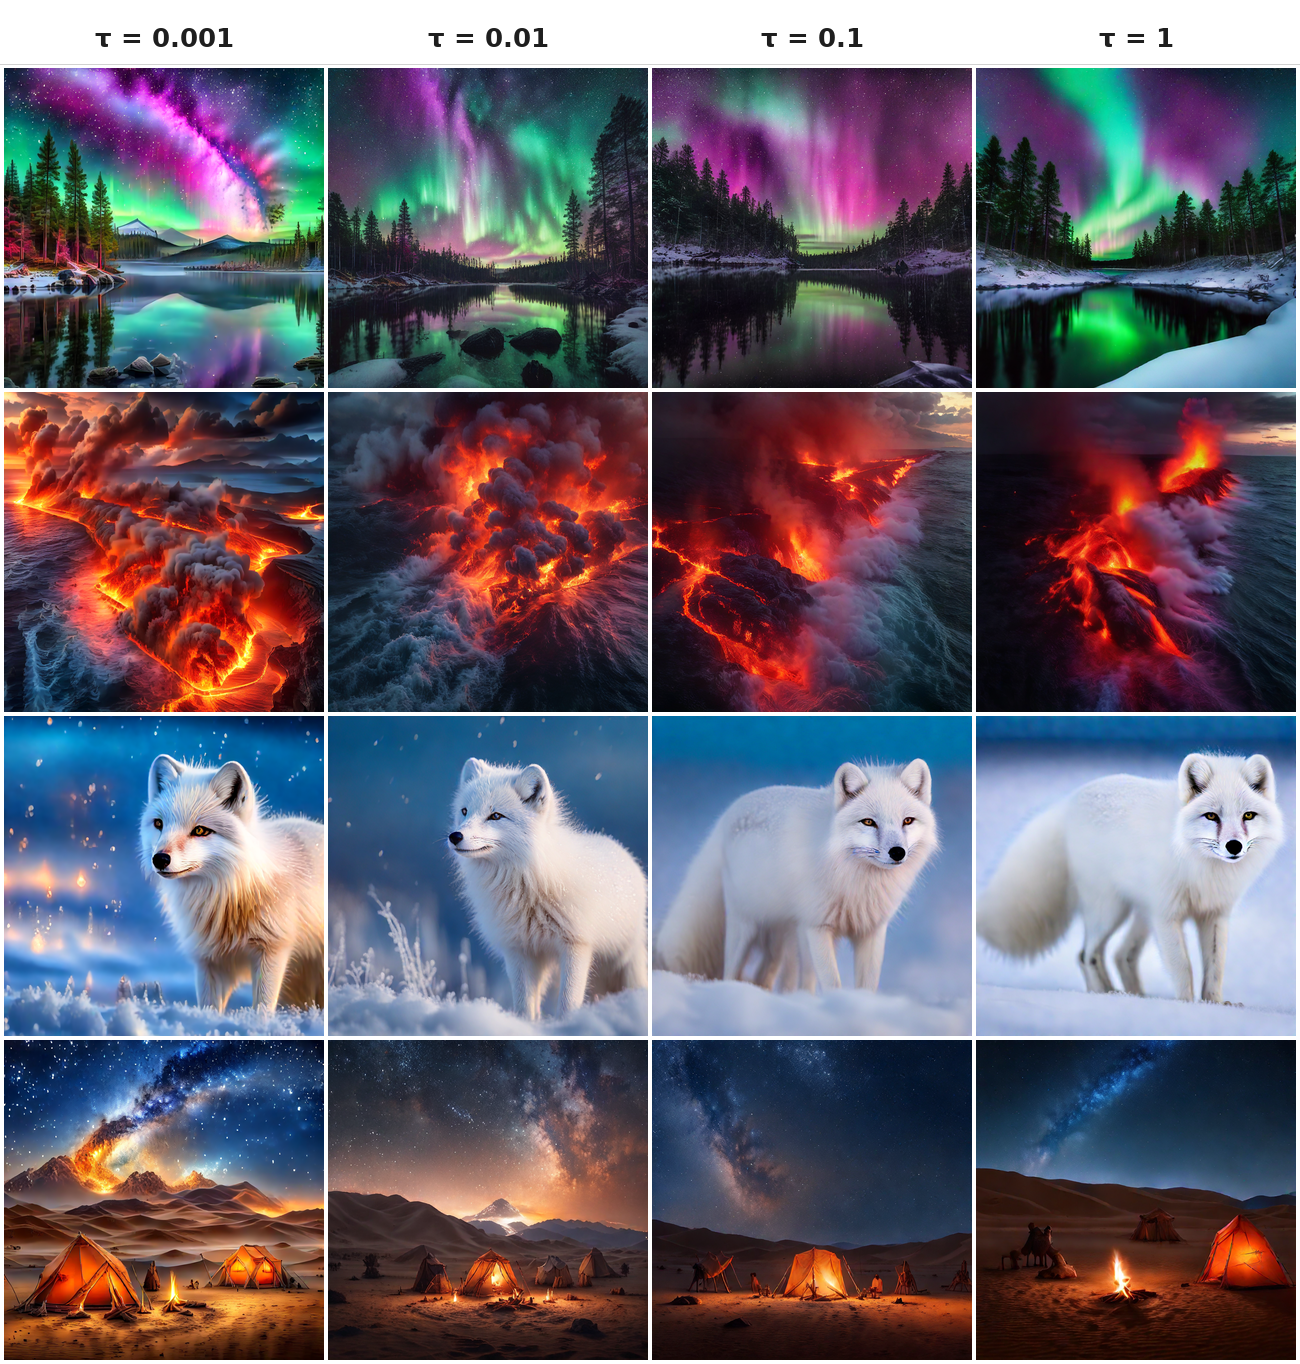
\includegraphics[width=\textwidth]{pictures/tau_figure.png}
\caption{\textbf{Qualitative effect of temperature $\tau$.} Images generated from the same prompt at decreasing $\tau$ (left to right). Smaller $\tau$ sharpens reward weighting and increases visual appeal, but introduces over-saturation and fine-detail artifacts at very low values, illustrating the preference--fidelity trade-off. Prompts in Appendix~\ref{app:prompts}.}
\label{fig:tau_ablation}
\end{figure}

\begin{figure}[h]
\centering
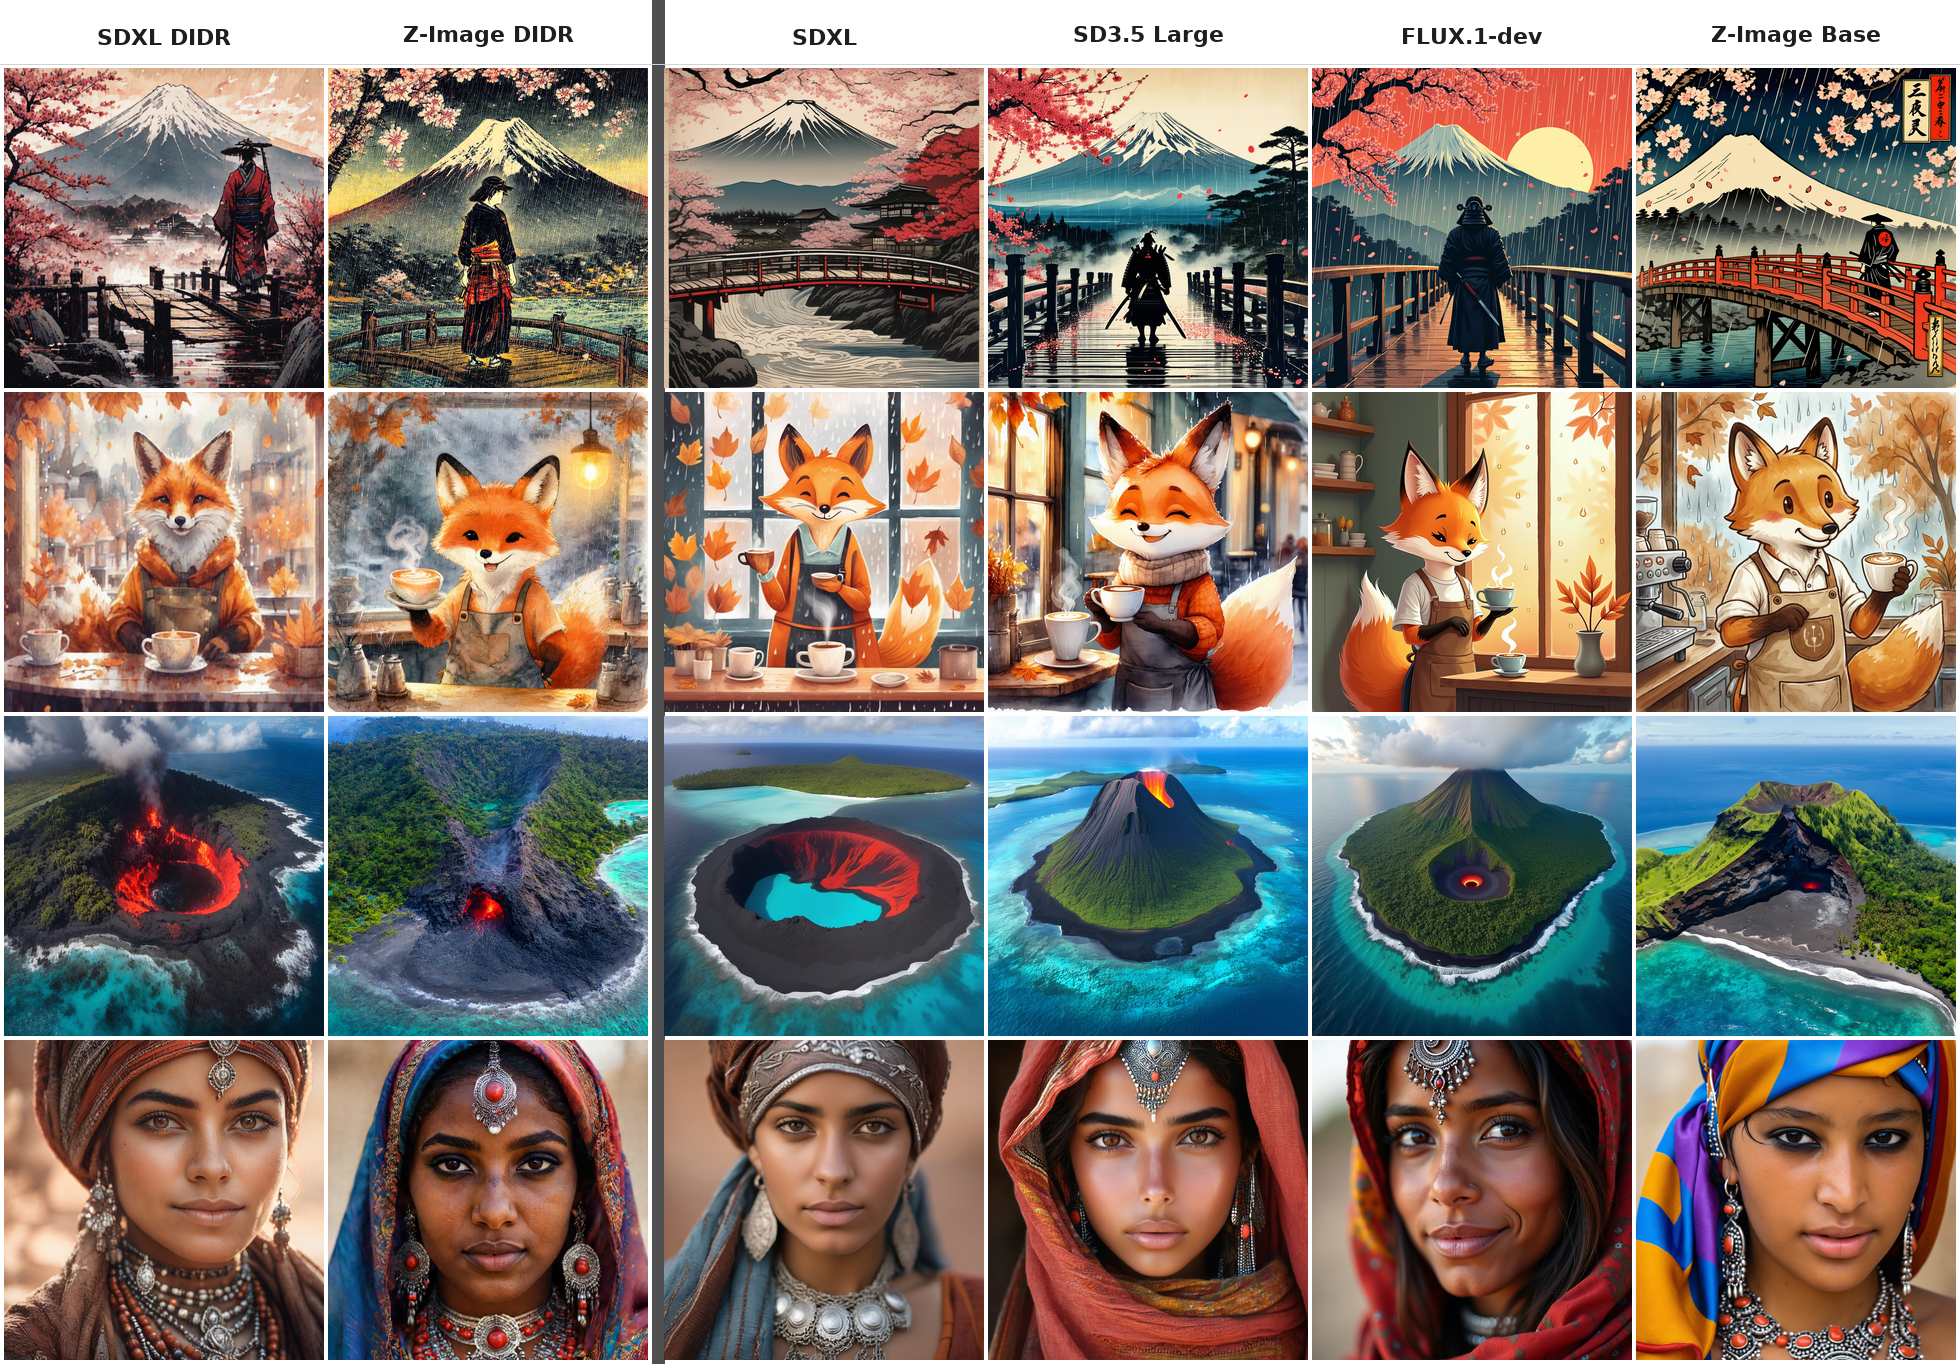
\includegraphics[width=\textwidth]{pictures/mult_figure.png}
\caption{\textbf{Qualitative comparison against multi-step baselines.} One-step \textsc{Didr} compared with 50-step SDXL, 50-step Z-Image, 50-step FLUX-dev, and 28-step SD3.5-Large on matched prompts. \textsc{Didr} achieves comparable or superior visual quality and prompt fidelity in a single inference step. Prompts in Appendix~\ref{app:prompts}.}
\label{fig:onestep_vs_multistep}
\end{figure}

\begin{figure}[h]
\centering
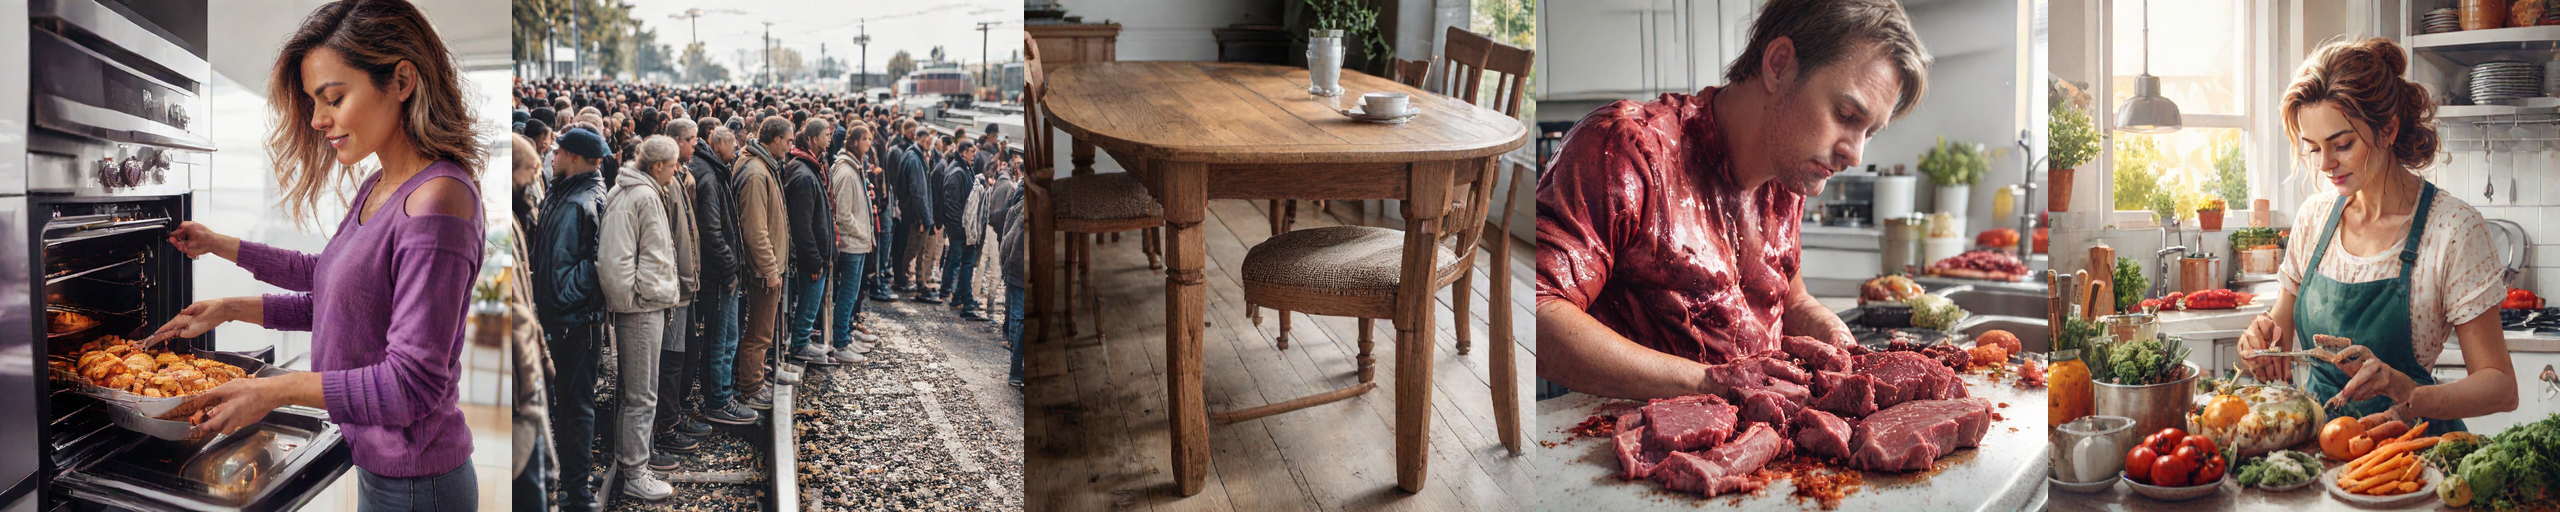
\includegraphics[width=\textwidth]{pictures/failure_figure.png}
\caption{\textbf{Failure cases of \textsc{Didr}:} anatomical errors, incorrect counts, structural distortions, and subject--background entanglement. Prompts in Appendix~\ref{app:prompts}.}
\label{fig:failure}
\end{figure}

\section{Theoretical Derivations}
\label{app:theory}

\subsection{Proof of the RLHF-Target Equivalence (Eq.~\eqref{eq:rlhf_kl})}
\label{app:proof_lem1}
\begin{proof}
Let $Z(c)\triangleq\int q_0(x_0|c)\exp(r(x_0,c)/\tau)\diff x_0<\infty$ and $q^*(x_0|c)\triangleq q_0(x_0|c)\exp(r/\tau)/Z(c)$. Expanding $\mathcal{L}(\theta)$:
\begin{align}
\mathcal{L}(\theta)
&= \tau\int p_\theta\!\left[\log p_\theta - \log q_0 - \frac{r}{\tau}\right]\diff x_0
= \tau\int p_\theta\!\left[\log p_\theta - \log\!\left(q_0\,e^{r/\tau}\right)\right]\diff x_0.
\end{align}
Since $q_0 e^{r/\tau} = Z(c)\,q^*$, this becomes $\tau\,\mathcal{D}_{\mathrm{KL}}(p_\theta\|q^*) - \tau\log Z(c)$. As $Z(c)$ is independent of $\theta$, the two objectives share the same minimizer.
\end{proof}

\subsection{Proof of Proposition~\ref{thm:ikl_equiv} (IKL Shares the RLHF Minimizer)}
\label{app:proof_thm_ikl_equiv}
\begin{proof}
\textbf{(i) Non-negativity.} Follows immediately from $\mathcal{D}_{\mathrm{KL}}\geq 0$ and $w(t)>0$.

\textbf{(ii) Convexity.} $\mathcal{D}_{\mathrm{KL}}(p\|q^*)$ is convex in $p$ for fixed $q^*$; a positively weighted integral of convex functionals is convex.

\textbf{(iii) Unique minimizer.} $\mathcal{L}_{\mathrm{IKL}}=0$ iff $\mathcal{D}_{\mathrm{KL}}(p_t\|q_t^*)=0$ for a.e.\ $t\in(0,T]$, since $w(t)>0$ and $\mathcal{D}_{\mathrm{KL}}=0$ iff the distributions coincide. This forces $p_t=q_t^*$ on a set of full measure in $(0,T]$, hence on a sequence $t_n\downarrow 0$. Since SDE marginals are weakly continuous in $t$ (standard for Lipschitz drift and diffusion coefficients), taking $n\to\infty$ gives $p_0=q_0^*=q^*$, which by Eq.~\eqref{eq:reward_tilted_target} is the unique minimizer of $\mathcal{L}$.
\end{proof}

\subsection{Proof of Theorem~\ref{thm:score_gradient} (Score-based DIDR Gradient)}
\label{app:proof_thm2}
\begin{proof}
Let $x_t = \mathcal{F}(g_\theta(z,c),\mathbf{w},t)$, $v_\theta\triangleq\partial x_t/\partial\theta$, and $s_\theta\triangleq\nabla_{x_t}\log p_{\theta,t}$. Differentiating $\mathcal{D}_{\mathrm{KL}}(p_{\theta,t}\|q_t^*)=\int p_{\theta,t}\log(p_{\theta,t}/q_t^*)\diff x_t$ in $\theta$:
\begin{equation}
\nabla_\theta\,\mathcal{D}_{\mathrm{KL}}(p_{\theta,t}\|q_t^*)
= \underbrace{\int\frac{\partial p_{\theta,t}}{\partial\theta}\log\frac{p_{\theta,t}}{q_t^*}\,\diff x_t}_{\mathrm{(I)}}
+ \underbrace{\int p_{\theta,t}\,\frac{\partial\log p_{\theta,t}}{\partial\theta}\,\diff x_t}_{\mathrm{(II)}}.
\end{equation}
Term (II) equals $\partial_\theta\!\int p_{\theta,t}\diff x_t = 0$.

\textbf{Continuity equation.} For any smooth test function $\phi$, differentiating both sides of $\E_{z,\mathbf{w}}[\phi(x_t)]=\int\phi\,p_{\theta,t}\diff x_t$ in $\theta$:
\begin{equation}
\int\phi\,\frac{\partial p_{\theta,t}}{\partial\theta}\diff x_t
= \E_{z,\mathbf{w}}\!\bigl[\nabla_{x_t}\phi(x_t)\cdot v_\theta\bigr]
= \int p_{\theta,t}\,\nabla_{x_t}\phi\cdot v_\theta\,\diff x_t
= -\int\phi\,\nabla_{x_t}\cdot(p_{\theta,t}\,v_\theta)\,\diff x_t,
\end{equation}
where the last step is integration by parts. Since $\phi$ is arbitrary,
\begin{equation}
\label{eq:continuity}
\frac{\partial p_{\theta,t}}{\partial\theta} = -\nabla_{x_t}\cdot(p_{\theta,t}\,v_\theta).
\end{equation}

\textbf{KL gradient.} Substituting \eqref{eq:continuity} into term (I) and integrating by parts:
\begin{align}
\mathrm{(I)}
&= -\int\nabla_{x_t}\cdot(p_{\theta,t}\,v_\theta)\,\log\frac{p_{\theta,t}}{q_t^*}\,\diff x_t \nonumber\\
&= \int p_{\theta,t}\,v_\theta\cdot\nabla_{x_t}\log\frac{p_{\theta,t}}{q_t^*}\,\diff x_t \nonumber\\
&= \int p_{\theta,t}\,v_\theta\cdot\bigl(s_\theta(x_t,t,c) - \nabla_{x_t}\log q_t^*(x_t|c)\bigr)\,\diff x_t.
\end{align}
Rewriting as an expectation over $(z,\mathbf{w})$ via $\int p_{\theta,t}\,\varphi\,\diff x_t = \E_{z,\mathbf{w}}[\varphi(x_t)]$ and substituting $v_\theta = \partial x_t/\partial\theta$:
\begin{equation}
\nabla_\theta\,\mathcal{D}_{\mathrm{KL}}(p_{\theta,t}\|q_t^*) = \E_{z,\mathbf{w}}\!\left[\bigl(s_\theta(x_t,t,c)-\nabla_{x_t}\log q_t^*(x_t|c)\bigr)\frac{\partial x_t}{\partial\theta}\right].
\end{equation}
Multiplying by $w(t)$, integrating over $t\in(0,T]$, and exchanging the $t$-integral with the expectation via Fubini gives Eq.~\eqref{eq:ikl_grad}.

\textbf{Target score decomposition} ($\nabla_{x_t}\log q_t^* = s_{\mathrm{ref}} + s_r$)\textbf{.}
Substituting $q^*(x_0|c) = q_0(x_0|c)\exp(r/\tau)/Z(c)$ into $q_t^*(x_t|c)=\int q_t(x_t|x_0)\,q^*(x_0|c)\diff x_0$ and using the Bayes factorization $q_0(x_0|c)\,q_t(x_t|x_0)=q_t(x_t|c)\,q(x_0|x_t,c)$:
\begin{align}
q_t^*(x_t|c)
&= \frac{1}{Z(c)}\int q_t(x_t|x_0)\,q_0(x_0|c)\exp\!\left(\frac{r(x_0,c)}{\tau}\right)\diff x_0 \nonumber\\
&= \frac{q_t(x_t|c)}{Z(c)}\int q(x_0|x_t,c)\exp\!\left(\frac{r(x_0,c)}{\tau}\right)\diff x_0 \nonumber\\
&= \frac{q_t(x_t|c)}{Z(c)}\;\E_{x_0\sim q(x_0|x_t,c)}\!\left[\exp\!\left(\frac{r(x_0,c)}{\tau}\right)\right].
\end{align}

Taking the logarithm of the factored form:
\begin{equation}
\log q_t^*(x_t|c) = \log q_t(x_t|c) + \log\E_{x_0\sim q(x_0|x_t,c)}\!\left[\exp\!\left(\frac{r(x_0,c)}{\tau}\right)\right] - \log Z(c).
\end{equation}
Applying $\nabla_{x_t}$: since $Z(c)$ does not depend on $x_t$, its gradient vanishes, giving
\begin{equation}
\nabla_{x_t}\log q_t^*(x_t|c)
= \underbrace{\nabla_{x_t}\log q_t(x_t|c)}_{=\,s_{\mathrm{ref}}(x_t,t,c)}
+ \underbrace{\nabla_{x_t}\log\E_{x_0\sim q(x_0|x_t,c)}\!\left[\exp\!\left(\frac{r(x_0,c)}{\tau}\right)\right]}_{\mathrm{DRS}(x_t,t,c)},
\end{equation}
which is exactly the decomposition in Eq.~\eqref{eq:ikl_grad}. The DRS term is intractable as written; Appendix~\ref{app:proof_lem4} derives a differentiable estimator for it.
\end{proof}

\subsection{Proof of Proposition~\ref{prop:drp} (Diffused Reward Proxy)}
\label{app:proof_lem4}
\begin{proof}
We derive a differentiable estimator for
\begin{equation}
\mathrm{DRS}(x_t,t,c)
= \nabla_{x_t}\log\E_{x_0\sim q(x_0|x_t,c)}\!\left[\exp\!\left(\frac{r(x_0,c)}{\tau}\right)\right].
\end{equation}

By the identity $\nabla\log f = \nabla f/f$:
\begin{equation}
\mathrm{DRS}(x_t,t,c)
= \frac{\nabla_{x_t}\,\E_{x_0\sim q(x_0|x_t,c)}\!\left[\exp\!\left(\tfrac{r(x_0,c)}{\tau}\right)\right]}
{\E_{\tilde x_0\sim q(\tilde x_0|x_t,c)}\!\left[\exp\!\left(\tfrac{r(\tilde x_0,c)}{\tau}\right)\right]}.
\end{equation}

To handle the numerator, we obtain differentiable approximate samples from the reference posterior $q(x_0|x_t,c)$ by running a denoising chain with the frozen reference model. Denote this map $x_0 = \mathcal{G}_{\mathrm{ref}}(x_t,\boldsymbol{\epsilon})$, initialized at $\hat{x}_{t_S}=x_t$, where $\boldsymbol{\epsilon}=(\epsilon^{(S)},\ldots,\epsilon^{(1)})$ is the sequence of injected noise vectors (empty for deterministic chains). The chain differs by model type:

\emph{VP diffusion (SDXL).} At each step $j=S,S{-}1,\ldots,1$, the Tweedie formula gives a clean-image estimate,
\[
\hat{x}_0^{(j)} = \frac{\hat{x}_{t_j}+\sigma_{t_j}^2\,s_{\mathrm{ref}}(\hat{x}_{t_j},t_j,c)}{\alpha_{t_j}},
\]
followed by a stochastic DDPM-style update
\[
\hat{x}_{t_{j-1}} = \alpha_{t_{j-1}}\hat{x}_0^{(j)} + \sigma_{t_{j-1}}\frac{\hat{x}_{t_j}-\alpha_{t_j}\hat{x}_0^{(j)}}{\sigma_{t_j}} + \tilde\sigma_{t_j}\,\epsilon^{(j)},
\qquad \epsilon^{(j)}\sim\mathcal{N}(0,I),
\]
where $\tilde\sigma_{t_j}=\sigma_{t_{j-1}}\sqrt{1-\dfrac{\alpha_{t_j}^2\,\sigma_{t_{j-1}}^2}{\alpha_{t_{j-1}}^2\,\sigma_{t_j}^2}}$ is the DDPM posterior standard deviation. Injecting independent noise $\epsilon^{(j)}$ for each of the $K$ chains yields $K$ diverse approximate posterior samples; the output of each chain is $\hat{x}_0^{(1)}$.

\emph{Flow matching (Z-Image).} A fixed Euler schedule yields identical $\hat{x}_0$ across all $K$ chains. Instead, each chain draws $S$ timesteps uniformly at random from $(0,t_S]$, runs the deterministic Euler ODE on its own schedule,
\[
\hat{x}_{t_{j-1}^{(k)}} = \hat{x}_{t_j^{(k)}} + \bigl(t_{j-1}^{(k)}-t_j^{(k)}\bigr)\,v_{\mathrm{ref}}\!\left(\hat{x}_{t_j^{(k)}},t_j^{(k)},c\right),
\]
and returns $\hat{x}_0^{(1)}=\hat{x}_{t_1^{(k)}}-t_1^{(k)}\,v_{\mathrm{ref}}(\hat{x}_{t_1^{(k)}},t_1^{(k)},c)$, yielding $K$ diverse approximate denoising endpoints induced by randomized discretization paths.

In both cases $\mathcal{G}_{\mathrm{ref}}$ is differentiable in $x_t$ for fixed $\boldsymbol{\epsilon}$, since all operations are compositions of smooth network evaluations and linear maps. Under this reparameterization the expectation becomes $\E_{\boldsymbol{\epsilon}}[\exp(r(\mathcal{G}_{\mathrm{ref}}(x_t,\boldsymbol{\epsilon}),c)/\tau)]$, in which $x_t$ enters explicitly through $\mathcal{G}_{\mathrm{ref}}$ rather than through the measure. Interchanging gradient and expectation via dominated convergence (justified when $r$ is smooth with bounded gradient and $\mathcal{G}_{\mathrm{ref}}$ is uniformly Lipschitz in $x_t$):
\begin{align}
\nabla_{x_t}\,\E_{x_0\sim q(x_0|x_t,c)}\!\left[\exp\!\left(\frac{r(x_0,c)}{\tau}\right)\right]
&= \E_{\boldsymbol{\epsilon}}\!\left[\nabla_{x_t}\exp\!\left(\frac{r(\mathcal{G}_{\mathrm{ref}}(x_t,\boldsymbol{\epsilon}),c)}{\tau}\right)\right].
\end{align}
Applying the chain rule:
\begin{equation}
\nabla_{x_t}\exp\!\left(\frac{r(\mathcal{G}_{\mathrm{ref}}(x_t,\boldsymbol{\epsilon}),c)}{\tau}\right)
= \exp\!\left(\frac{r(x_0,c)}{\tau}\right)\cdot\frac{1}{\tau}\underbrace{\frac{\partial r(x_0,c)}{\partial x_0}\frac{\partial\mathcal{G}_{\mathrm{ref}}(x_t,\boldsymbol{\epsilon})}{\partial x_t}}_{\triangleq\;\nabla_{x_t}r(x_0,c)},
\end{equation}
where $\nabla_{x_t}r(x_0,c)$ denotes the pathwise gradient of $r$ through the differentiable denoising chain. Converting back to the $q(x_0|x_t,c)$ expectation:
\begin{equation}
\nabla_{x_t}\,\E_{x_0\sim q(x_0|x_t,c)}\!\left[\exp\!\left(\frac{r(x_0,c)}{\tau}\right)\right]
= \E_{x_0\sim q(x_0|x_t,c)}\!\left[\exp\!\left(\frac{r(x_0,c)}{\tau}\right)\cdot\frac{1}{\tau}\nabla_{x_t}r(x_0,c)\right].
\end{equation}

Dividing numerator and denominator:
\begin{equation}
\mathrm{DRS}(x_t,t,c)
= \E_{x_0\sim q(x_0|x_t,c)}\!\left[
\frac{\exp\!\left(\tfrac{r(x_0,c)}{\tau}\right)}
{\E_{\tilde x_0\sim q(\tilde x_0|x_t,c)}\!\left[\exp\!\left(\tfrac{r(\tilde x_0,c)}{\tau}\right)\right]}
\cdot\frac{1}{\tau}\nabla_{x_t}r(x_0,c)
\right],
\end{equation}
which is precisely the softmax-weighted gradient estimator in Eq.~\eqref{eq:drp_estimator}.
\end{proof}

\begin{remark}[Regularity assumptions]
The interchange of gradient and expectation above requires: (i) $r$ is smooth with bounded gradient, and (ii) $\mathcal{G}_{\mathrm{ref}}$ is uniformly Lipschitz in $x_t$. Condition~(i) holds for standard differentiable reward models such as PickScore. Condition~(ii) holds because $\mathcal{G}_{\mathrm{ref}}$ is a finite composition of smooth network evaluations and linear maps, hence globally Lipschitz on any compact domain.
\end{remark}

\subsection{A Bimodal Gaussian Example of Terminal Reward Domination}
\label{app:reward_domination_gaussian}

All results below hold under the mild assumption that the two modes are well-separated ($\mu/\sigma\gg 1$), in which regime $\Phi(-\mu/\sigma)\approx 0$ and every approximation becomes exact as $\mu/\sigma\to\infty$. The $\approx$ symbol denotes equality up to corrections of order $\Phi(-\mu/\sigma)$.

\paragraph{Setup.}
Consider the bimodal reference
\[
p_0
=
\tfrac12\mathcal N(-\mu,\sigma^2)
+
\tfrac12\mathcal N(\mu,\sigma^2),
\qquad
\mu>\sigma>0,
\]
the generator family
\[
q_{\alpha,0}
=
(1-\alpha)\mathcal N(-\mu,\sigma^2)
+
\alpha\mathcal N(\mu,\sigma^2),
\qquad
\alpha\in[0,1],
\]
and the binary reward $r(x_0)=\mathbf 1[x_0>0]$.

\paragraph{Exact reward expectation.}
By direct computation,
\begin{align}
\E_{q_{\alpha,0}}[r]
&= (1-\alpha)\,P\!\bigl(\mathcal N(-\mu,\sigma^2)>0\bigr)
+\alpha\,P\!\bigl(\mathcal N(\mu,\sigma^2)>0\bigr) \nonumber\\
&= (1-\alpha)\,\Phi\!\left(-\tfrac{\mu}{\sigma}\right)
+\alpha\,\Phi\!\left(\tfrac{\mu}{\sigma}\right)
= \alpha + (1-2\alpha)\,\Phi\!\left(-\tfrac{\mu}{\sigma}\right),
\end{align}
where $\Phi$ is the standard normal CDF. Since $\Phi(-\mu/\sigma)\to 0$ as $\mu/\sigma\to\infty$,
\[
\E_{q_{\alpha,0}}[r] \approx \alpha,
\qquad
\frac{d}{d\alpha}\E_{q_{\alpha,0}}[r]\big|_{\alpha=1} = 1 - 2\Phi\!\left(-\tfrac{\mu}{\sigma}\right) \approx 1.
\]

\paragraph{Forward marginals.}
Under the VP forward process with $\bar\alpha_t=e^{-\gamma t}$, $t\in[0,\infty)$, the forward kernel is $q_t(x_t|x_0)=\mathcal{N}(x_t;\sqrt{\bar\alpha_t}\,x_0,(1-\bar\alpha_t)I)$, so the marginals are
\[
q_{\alpha,t}
=
(1-\alpha)\phi_{-,t}
+
\alpha\phi_{+,t},
\qquad
p_t
=
\tfrac12\phi_{-,t}
+
\tfrac12\phi_{+,t},
\]
where $\phi_{\pm,t}=\mathcal N(\pm m_t,\Sigma_t)$ with
\[
m_t=\sqrt{\bar\alpha_t}\,\mu,
\qquad
\Sigma_t=1-\bar\alpha_t(1-\sigma^2).
\]

\paragraph{Objective and convexity.}
The endpoint-reward objective (to be \emph{minimized}) is
\[
\mathcal{L}_{\rm term}(\alpha)
=
-\E_{q_{\alpha,0}}[r]
+
\tau\int_0^\infty
D_t(\alpha)\,\diff t,
\qquad
D_t(\alpha):=
\mathrm{KL}(q_{\alpha,t}\|p_t).
\]
Since $q_{\alpha,t}$ is affine in $\alpha$ and KL divergence is convex in its first argument, $D_t(\alpha)$ is convex in $\alpha$, and $-\E_{q_{\alpha,0}}[r]$ is linear in $\alpha$. Hence $\mathcal{L}_{\rm term}$ is convex in $\alpha$, so $\mathcal{L}_{\rm term}'$ is non-decreasing on $[0,1]$. Consequently, $\alpha^*=1$ (collapse to the positive mode) occurs whenever the left derivative satisfies
\[
\mathcal{L}_{\rm term}'(1^-)\le 0,
\]
since convexity then forces $\mathcal{L}_{\rm term}'(\alpha)\le\mathcal{L}_{\rm term}'(1^-)\le 0$ for all $\alpha\in[0,1)$, making $\mathcal{L}_{\rm term}$ non-increasing throughout and the minimum attained at $\alpha^*=1$.

\paragraph{Computing $D_t'(1)$.}
Differentiating $D_t(\alpha)=\mathrm{KL}(q_{\alpha,t}\|p_t)$ with respect to $\alpha$ and using $\partial_\alpha q_{\alpha,t}=\phi_{+,t}-\phi_{-,t}$ (together with the fact that $\partial_\alpha\int q_{\alpha,t}\,\diff x=0$, so the term from differentiating the $\log q_{\alpha,t}$ factor vanishes by normalization), we obtain
\[
D_t'(\alpha)
=
\int
(\phi_{+,t}-\phi_{-,t})\,
\log\frac{q_{\alpha,t}(x)}{p_t(x)}
\,\diff x.
\]
At $\alpha=1$, $q_{1,t}=\phi_{+,t}$, so
\[
D_t'(1)
=
\int
(\phi_{+,t}(x)-\phi_{-,t}(x))\,
\log\frac{\phi_{+,t}(x)}{\frac12(\phi_{+,t}(x)+\phi_{-,t}(x))}
\,\diff x.
\]
Since $\phi_{\pm,t}=\mathcal{N}(\pm m_t,\Sigma_t)$, the Gaussian log-ratio is
\[
\log\frac{\phi_{+,t}(x)}{\phi_{-,t}(x)}
=
-\frac{(x-m_t)^2-(x+m_t)^2}{2\Sigma_t}
=
\frac{2m_t x}{\Sigma_t},
\]
so $\phi_{-,t}(x)/\phi_{+,t}(x)=\exp(-2m_t x/\Sigma_t)$. Substituting:
\[
\log\frac{\phi_{+,t}(x)}{\frac12(\phi_{+,t}+\phi_{-,t})}
=
\log\frac{2}{1+e^{-2m_tx/\Sigma_t}}.
\]

We now simplify by symmetry. Split the integral into contributions from $\phi_{+,t}$ and $\phi_{-,t}$:
\[
D_t'(1)
=
\int\phi_{+,t}(x)\,\log\frac{2}{1+e^{-2m_tx/\Sigma_t}}\,\diff x
-
\int\phi_{-,t}(x)\,\log\frac{2}{1+e^{-2m_tx/\Sigma_t}}\,\diff x.
\]
In the second integral, substitute $x\mapsto -x$; since $\phi_{-,t}(-x)=\phi_{+,t}(x)$:
\[
\int\phi_{-,t}(x)\,\log\frac{2}{1+e^{-2m_tx/\Sigma_t}}\,\diff x
=
\int\phi_{+,t}(x)\,\log\frac{2}{1+e^{2m_tx/\Sigma_t}}\,\diff x.
\]
Combining both integrals:
\begin{equation}
\label{eq:Dt_prime_1}
D_t'(1)
=
\int\phi_{+,t}(x)\,\log\frac{1+e^{2m_tx/\Sigma_t}}{1+e^{-2m_tx/\Sigma_t}}\,\diff x
=
\E_{x\sim\phi_{+,t}}\!\left[\log\frac{1+e^{2m_tx/\Sigma_t}}{1+e^{-2m_tx/\Sigma_t}}\right].
\end{equation}

Finally, we invoke the well-separated assumption. Define $a_t\triangleq m_t/\sqrt{\Sigma_t}$. Under $\phi_{+,t}=\mathcal{N}(m_t,\Sigma_t)$, a typical sample satisfies $x\approx m_t$, so $2m_t x/\Sigma_t\approx 2m_t^2/\Sigma_t=2a_t^2$. In the regime $\mu/\sigma\gg1$ (so $a_t\gg1$ for all $t$ where the diffusion has not yet erased the modes), $e^{2m_tx/\Sigma_t}\gg1$ and $e^{-2m_tx/\Sigma_t}\approx0$ throughout the support of $\phi_{+,t}$. Therefore,
\[
\log\frac{1+e^{2m_tx/\Sigma_t}}{1+e^{-2m_tx/\Sigma_t}}
\approx
\log e^{2m_tx/\Sigma_t}
=
\frac{2m_t x}{\Sigma_t}.
\]
Substituting into Eq.~\eqref{eq:Dt_prime_1} and using $\E_{x\sim\phi_{+,t}}[x]=m_t$:
\[
D_t'(1)
\approx
\E_{x\sim\phi_{+,t}}\!\left[\frac{2m_t x}{\Sigma_t}\right]
=
\frac{2m_t}{\Sigma_t}\,\E_{x\sim\phi_{+,t}}[x]
=
\frac{2m_t^2}{\Sigma_t}.
\]

\paragraph{Collapse condition.}
Combining the derivative of the reward term ($\approx -1$ after negation) and the regularizer:
\[
\mathcal{L}_{\rm term}'(1)
\approx
-1
+
\tau\int_0^\infty
\frac{2m_t^2}{\Sigma_t}\,\diff t.
\]
The condition $\mathcal{L}_{\rm term}'(1)\le0$ gives the collapse threshold
\[
\tau
\le
\frac{1}{B_{\rm crit}},
\qquad
B_{\rm crit}
\triangleq
\int_0^\infty
\frac{2m_t^2}{\Sigma_t}\,\diff t.
\]

\paragraph{Closed-form evaluation of $B_{\rm crit}$.}
Substituting $m_t^2=\bar\alpha_t\mu^2$ and $\Sigma_t=1-\bar\alpha_t(1-\sigma^2)$:
\[
B_{\rm crit}
=
\int_0^\infty
\frac{2\mu^2\,e^{-\gamma t}}
{1-e^{-\gamma t}(1-\sigma^2)}
\,\diff t.
\]
Change variables $u=e^{-\gamma t}$, so $\diff u=-\gamma u\,\diff t$ and the limits $t:0\to\infty$ become $u:1\to 0$:
\[
B_{\rm crit}
=
\int_1^0
\frac{2\mu^2\,u}
{1-(1-\sigma^2)u}
\cdot\frac{-\diff u}{\gamma u}
=
\frac{2\mu^2}{\gamma}
\int_0^1
\frac{\diff u}{1-(1-\sigma^2)u}.
\]
For $\sigma^2\neq1$, the integral evaluates via $\int_0^1\frac{\diff u}{1-cu}=\frac{-\log(1-c)}{c}$ with $c=1-\sigma^2$:
\[
B_{\rm crit}
=
\frac{2\mu^2}{\gamma}\cdot\frac{-\log\sigma^2}{1-\sigma^2}.
\]
Therefore, the collapse condition is
\[
\boxed{
\tau
\le
\frac{\gamma(1-\sigma^2)}{2\mu^2(-\log\sigma^2)}
\quad
\Longrightarrow
\quad
\alpha^*=1.
}
\]
The case $\sigma^2=1$ follows by L'H\^opital's rule (or a direct integral): $\int_0^1 \diff u/(1-0)=1$, giving
\[
\boxed{
\tau\le \frac{\gamma}{2\mu^2}
\quad
\Longrightarrow
\quad
\alpha^*=1.
}
\]

This shows that terminal reward domination occurs under the integral forward KL penalty for any finite $\tau$ below a closed-form threshold. Larger $\gamma$ (faster diffusion) raises the critical $\tau$, making collapse to the rewarded mode easier to trigger at any fixed regularization strength.

\section{1-D Toy Experiment}
\label{app:toy_experiment}

This section describes the setup for the 1-D empirical validation of terminal reward domination (Figure~\ref{fig:schematic_combined}(b)).

\paragraph{Reference distribution and reward.}
The reference is a symmetric bimodal Gaussian
\[
q_0 = \tfrac{1}{2}\mathcal{N}(-\mu,\sigma^2) + \tfrac{1}{2}\mathcal{N}(\mu,\sigma^2), \qquad \mu=2,\;\sigma=0.5,
\]
with ideal binary reward $r_{\mathrm{hard}}(x)=\mathbf{1}[x>0]$. For gradient-based training, we use the smooth approximation
\[
r(x)=\operatorname{sigmoid}(\beta x), \qquad \beta=20,
\]
so that $r(x)$ approximates $r_{\mathrm{hard}}(x)$ except in a narrow neighborhood of the decision boundary while remaining differentiable.

\paragraph{Forward process.}
VP diffusion with rate $\gamma=20$: $\bar\alpha_t=e^{-\gamma t}$, $t\in[0,T]$, $T=0.25$, giving $\bar\alpha_T=e^{-5}\approx0.007$. This places the experiment firmly in the collapse regime: the closed-form domination threshold derived in Appendix~\ref{app:reward_domination_gaussian} evaluates to $\tau_{\mathrm{crit}}\approx1.35>\tau=1$.

\paragraph{Networks.}
Both $s_{\mathrm{ref}}$ and $s_\psi$ are MLPs with input $(x,t)\in\mathbb{R}^2$, three hidden layers of width~128, SiLU activations, and a scalar output (noise-prediction parameterisation; converted to score via $s=-\hat{\varepsilon}/\sqrt{1-\bar\alpha_t}$).
The generator $g_\theta:\mathcal{N}(0,1)\to\mathbb{R}$ uses the same architecture with a scalar input $z$.

\paragraph{Training pipeline.}
\begin{enumerate}[1.]
    \item \textbf{Reference model.} $s_{\mathrm{ref}}$ is trained for 10{,}000 steps via DSM on samples from $q_0$ (Adam, lr=$3\times10^{-4}$, batch~2{,}048). Weights are frozen afterwards.
    \item \textbf{Generator distillation.} $g_\theta$ is initialised by regressing against 30-step DDIM samples from $s_{\mathrm{ref}}$ using matched noise (3{,}000 steps, Adam, lr=$10^{-3}$, batch~2{,}048).
    \item \textbf{Teaching Assistant initialisation.} $s_\psi$ is copied from $s_{\mathrm{ref}}$ and fine-tuned during alignment.
    \item \textbf{Alignment.} 6{,}000 outer steps; each step runs 5 TA DSM updates (Adam, lr=$3\times10^{-4}$) followed by one generator update (Adam, lr=$10^{-4}$, batch~2{,}048). The two methods differ only in $s_{\mathrm{target}}$:
\end{enumerate}

\begin{center}
\begin{tabular}{ll}
\toprule
Method & Reward location \\
\midrule
DI++ & endpoint $x_0$ only \\
\textsc{Didr} & every noise level via DRS \\
\bottomrule
\end{tabular}
\end{center}

\paragraph{Evaluation.}
Final generators are evaluated on $n=10{,}000$ samples using the hard decision boundary $x>0$. For the ideal binary reward $r_{\mathrm{hard}}$, the theoretical optimal weight under $q^*$ is $P_{q^*}(x>0)=\operatorname{sigmoid}(1/\tau)\approx0.731$.
DI++ collapses to $P(x>0)\approx1$ while \textsc{Didr} converges to $P(x>0)\approx0.73$, confirming the theory.

\section{Evaluation Metrics}
\label{app:evaluation_metrics}

We use automatic metrics that measure complementary aspects of text-to-image generation. Preference metrics estimate human visual preference or aesthetics; text-alignment metrics measure whether the image satisfies the prompt; FID measures distributional fidelity against real images. For all metrics except FID, higher is better.

\paragraph{Preference metrics.}
PickScore~\citep{pickscore} is a CLIP-based human preference model trained on Pick-a-Pic pairwise user preferences, and is also the reward used for \textsc{Didr} training. ImageReward~\citep{xu2023imagereward} is a learned image-text reward model trained from human preference annotations for text-to-image outputs. HPSv2.1~\citep{hpsv2} evaluates human preference using the Human Preference Score benchmark and reports results over its standard prompt categories. Aesthetic Score~\citep{laionaes} uses the LAION aesthetic predictor, which estimates visual appeal from CLIP image embeddings and does not directly measure prompt faithfulness.

\paragraph{Text-alignment metrics.}
CLIPScore \citep{hessel2021clipscore,radford2021learning} measures image--text compatibility using CLIP embedding similarity. DPG-Bench \citep{dpgbench} evaluates semantic adherence on dense prompts containing multiple attributes and relations. GenEval \citep{geneval} is an object-focused benchmark that checks compositional correctness, including object presence, counting, color binding, position, and attribute relations.

\paragraph{Fidelity metric.}
FID~\citep{heusel2017gans} compares generated and real image distributions in Inception feature space:
\[
\mathrm{FID}
= \|\mu_r-\mu_g\|_2^2
+ \operatorname{Tr}\!\left(\Sigma_r+\Sigma_g-2(\Sigma_r\Sigma_g)^{1/2}\right),
\]
where $(\mu_r,\Sigma_r)$ and $(\mu_g,\Sigma_g)$ are Gaussian approximations of real and generated feature distributions. Lower FID indicates closer distributional match to the reference images, but it does not directly measure prompt alignment or human preference.

\section{Per-Category Results}
\label{app:geneval}

Tables~\ref{tab:geneval} and~\ref{tab:hpsv2} provide per-category breakdowns of GenEval and HPSv2.1 scores respectively. On GenEval, \textsc{Didr} achieves the highest overall score among one-step SDXL methods, with particularly strong gains on counting ($0.513$ vs.\ $0.428$ for DI*) and color attribute binding ($0.245$ vs.\ $0.215$). On HPSv2.1, \textsc{Didr}$_{\text{longer}}$ leads across all four style categories. For the Z-Image backbone, \textsc{zimage-Didr} improves substantially over the 1-step Z-Image-Turbo initialization (row marked $^\dagger$) on all categories, suggesting that the gains come from the alignment procedure rather than initialization quality.

\begin{table*}[!h]
\centering
\caption{GenEval per-category breakdown. \textbf{Bold}: best result within each one-step group. $^\dagger$: Z-Image-Turbo at 1~NFE (unofficial; \textsc{Didr} training initialization only). $-$: not reported.}
\label{tab:geneval}
\resizebox{\textwidth}{!}{\begin{tabular}{lclcccccccc}
\toprule
& & & & \multicolumn{6}{c}{\textbf{GenEval Category} $\uparrow$} & \\
\cmidrule(lr){5-10}
\textbf{Model} & \textbf{Steps} & \textbf{Arch.} & \textbf{Params} & \textbf{Single Obj.} & \textbf{Two Obj.} & \textbf{Counting} & \textbf{Colors} & \textbf{Color Attr.} & \textbf{Position} & \textbf{Overall} $\uparrow$ \\
\midrule
\multicolumn{11}{l}{\textit{Multi-step reference}} \\
SDXL~\citep{podell2023sdxl}           & 50 & UNet & 2.6B & 0.973 & 0.745 & 0.381 & 0.847 & 0.218 & 0.142 & 0.551 \\
SDXL-DPO~\citep{wallace2024diffusion} & 50 & UNet & 2.6B & 0.971 & 0.751 & 0.374 & 0.843 & 0.221 & 0.134 & 0.549 \\
SD3.5-large~\citep{sd35}              & 28 & DiT  & 8B   & 0.997 & 0.921 & 0.668 & 0.853 & 0.593 & 0.270 & 0.717 \\
FLUX-dev~\citep{fluxdev}              & 50 & DiT  & 12B  & 0.991 & 0.863 & 0.683 & 0.771 & 0.489 & 0.235 & 0.672 \\
Z-Image~\citep{zimage}                & 50 & DiT  & 6B   & 1.000 & 0.943 & 0.781 & 0.928 & 0.624 & 0.764 & 0.840 \\
\midrule
\multicolumn{11}{l}{\textit{One-step SDXL}} \\
SDXL DMD2~\citep{yin2024improved}                & 1 & UNet & 2.6B & 0.984 & 0.677 & 0.472 & 0.878 & 0.220 & \textbf{0.110} & 0.557 \\
SDXL Diff-Instruct~\citep{Luo2023DiffInstructAU} & 1 & UNet & 2.6B & 0.994 & 0.748 & 0.456 & 0.883 & 0.188 & 0.090 & 0.560 \\
SDXL Diff-Instruct++~\citep{anonymous2024diffinstruct} & 1 & UNet & 2.6B & 0.988 & 0.735 & 0.475 & 0.872 & 0.200 & 0.093 & 0.560 \\
SDXL Diff-Instruct*~\citep{luo2024onestep}       & 1 & UNet & 2.6B & 0.994 & 0.740 & 0.428 & 0.851 & 0.215 & 0.105 & 0.555 \\
\textbf{SDXL \textsc{Didr} (Ours)}                      & 1 & UNet & 2.6B & 0.991 & 0.727 & \textbf{0.513} & \textbf{0.891} & \textbf{0.245} & 0.108 & \textbf{0.579} \\
\textbf{SDXL \textsc{Didr}$_{\text{longer}}$ (Ours)}    & 1 & UNet & 2.6B & \textbf{1.000} & \textbf{0.758} & 0.472 & 0.883 & 0.190 & 0.095 & 0.566 \\
\midrule
\multicolumn{11}{l}{\textit{Z-Image backbone}} \\
Z-Image-Turbo~\citep{zimage}                     & 8 & DiT & 6B & \textbf{1.000} & \textbf{0.904} & \textbf{0.728} & \textbf{0.835} & \textbf{0.578} & \textbf{0.455} & \textbf{0.750} \\
\textbf{Z-Image \textsc{Didr} (Ours)}            & 1 & DiT & 6B & 0.997 & 0.846 & 0.625 & 0.811 & 0.533 & 0.340 & 0.692 \\
\hdashline
Z-Image-Turbo$^\dagger$~\citep{zimage}           & 1 & DiT & 6B & 0.972 & 0.513 & 0.559 & 0.795 & 0.300 & 0.293 & 0.572 \\
\bottomrule
\end{tabular}}
\end{table*}

\subsection*{HPSv2.1 Per-Category Results}
\label{app:hpsv2}

\begin{table*}[!t]
\centering
\caption{HPSv2.1 per-category breakdown. Same conventions as Table~\ref{tab:main}. $^\dagger$: Z-Image-Turbo at 1~NFE (unofficial; \textsc{Didr} training initialization only).}
\label{tab:hpsv2}
\resizebox{\textwidth}{!}{\begin{tabular}{lclcccccc}
\toprule
& & & & \multicolumn{5}{c}{\textbf{HPSv2.1} $\uparrow$} \\
\cmidrule(lr){5-9}
\textbf{Model} & \textbf{Steps} & \textbf{Arch.} & \textbf{Params} & \textbf{Animation} & \textbf{Concept-Art} & \textbf{Painting} & \textbf{Photo} & \textbf{Average} \\
\midrule
\multicolumn{9}{l}{\textit{Multi-step reference}} \\
SDXL~\citep{podell2023sdxl}            & 50 & UNet & 2.6B & 30.89 & 29.16 & 28.91 & 26.97 & 28.98 \\
SDXL-DPO~\citep{wallace2024diffusion}  & 50 & UNet & 2.6B & 32.08 & 30.80 & 30.82 & 28.12 & 30.45 \\
SD3.5-large~\citep{sd35}               & 28 & DiT  & 8B   & 31.87 & 30.05 & 30.31 & 28.01 & 30.06 \\
FLUX-dev~\citep{fluxdev}               & 50 & DiT  & 12B  & 31.95 & 30.35 & 31.21 & 29.10 & 30.65 \\
Z-Image~\citep{zimage}                 & 50 & DiT  & 6B   & 32.53    & 30.42    & 29.58    & 29.76    & 30.57 \\
\midrule
\multicolumn{9}{l}{\textit{One-step SDXL}} \\
SDXL DMD2~\citep{yin2024improved}                  & 1 & UNet & 2.6B & 31.53 & 29.86 & 29.43 & 29.14 & 29.99 \\
SDXL Diff-Instruct~\citep{Luo2023DiffInstructAU}   & 1 & UNet & 2.6B & 32.78 & 31.39 & 31.29 & 30.59 & 31.51 \\
SDXL Diff-Instruct++~\citep{anonymous2024diffinstruct} & 1 & UNet & 2.6B & 32.74 & 31.42 & 31.20 & 30.41 & 31.44 \\
SDXL Diff-Instruct*~\citep{luo2024onestep}          & 1 & UNet & 2.6B & 35.10 & 33.63 & 33.14 & 31.28 & 33.29 \\
\textbf{SDXL \textsc{Didr} (Ours)}                  & 1 & UNet & 2.6B & 35.64 & 34.21 & 33.81 & 31.41 & 33.77 \\
\textbf{SDXL \textsc{Didr}$_{\text{longer}}$ (Ours)} & 1 & UNet & 2.6B & \textbf{35.76} & \textbf{34.43} & \textbf{33.83} & \textbf{31.53} & \textbf{33.89} \\
\midrule
\multicolumn{9}{l}{\textit{Z-Image backbone}} \\
Z-Image-Turbo~\citep{zimage}                        & 8 & DiT & 6B & \textbf{33.44} & \textbf{31.99} & \textbf{31.26} & \textbf{30.76} & \textbf{31.86} \\
\textbf{Z-Image \textsc{Didr} (Ours)}               & 1 & DiT & 6B & 33.39 & 31.62 & 30.38 & 30.21 & 31.40 \\
\hdashline
Z-Image-Turbo$^\dagger$~\citep{zimage}              & 1 & DiT & 6B & 26.50 & 24.22 & 23.63 & 23.81 & 24.54 \\
\bottomrule
\end{tabular}}
\end{table*}

\section{Full Training Algorithm}
\label{app:alg_detail}

Algorithm~\ref{alg:didr_detail} provides the complete pseudocode for \textsc{Didr}, expanding the concise version in Algorithm~\ref{alg:didr}. The outer loop alternates between two stages. Stage~I updates the Teaching Assistant $s_\psi$ via denoising score matching to track the generator's current marginals. Stage~II updates the generator $g_\theta$: for each training step it samples a prompt and noise, forward-diffuses the generated image to a random time $t$, draws $K$ posterior samples via $S$-step reference denoising, computes the DRP estimate $s_r$ as a softmax-weighted gradient, and applies the IKL gradient. The CFG-corrected reference score $\tilde{s}_{\mathrm{ref}}$ is used throughout to maintain text alignment.

\begin{algorithm}[H]
\caption{\textsc{Didr}: Diff-Instruct with Diffused Reward (full pseudocode)}
\label{alg:didr_detail}
\SetAlgoLined
\SetKwInOut{Input}{Input}
\small
\Input{
prompt dataset $\mathcal{C}$; generator $g_\theta$; prior $p_z$;
reward model $r(\cdot, c)$; CFG scale $\cfg$;
reference diffusion $s_{\mathrm{ref}}$; Teaching Assistant (TA) $s_\psi$;
posterior samples $K$; temperature $\tau$; denoising steps $S$;
TA update rounds $K_{\mathrm{TA}}$; weights $w(t), \lambda(t)$.
}

\While{\textnormal{not converged}}{
\textbf{Stage I: Update Teaching Assistant (TA)}\;
\For{$k=1$ \KwTo $K_{\mathrm{TA}}$}{
Sample $c \sim \mathcal{C}, z \sim p_z, t \sim \pi(t)$\;
Generate $x_0 = g_\theta(z, c)$, diffuse $x_t \sim p_t(x_t|x_0)$\;
Update $\psi$ by minimizing DSM loss: $\mathcal{L}(\psi) = \lambda(t)\,\| s_\psi(x_t, t, c) - \nabla_{x_t} \log p_t(x_t|x_0) \|_2^2$\;
}

\BlankLine
\textbf{Stage II: Update Generator}\;
Sample $c \sim \mathcal{C}, z \sim p_z, t \sim \pi(t)$\;
Generate $x_0 = g_\theta(z, c)$, diffuse $x_t \sim p_t(x_t|x_0)$\;
Compute CFG score: $\tilde{s}_{\mathrm{ref}} = s_{\mathrm{ref}}(x_t,t,\emptyset) + \cfg\left[s_{\mathrm{ref}}(x_t,t,c) - s_{\mathrm{ref}}(x_t,t,\emptyset)\right]$\;
\BlankLine
\textit{Compute DRP estimate $s_r$ via posterior sampling:}\;
\For{$k=1$ \KwTo $K$}{
Run $S$-step differentiable denoising from $x_t$: $\hat{x}_0^{(k)} \leftarrow \mathrm{Denoise}_S(x_t, s_{\mathrm{ref}}, c)$\;
Compute $r^{(k)} = r(\hat{x}_0^{(k)}, c)$ and pathwise gradient $\nabla_{x_t} r^{(k)}$\;
}
Compute softmax weights: $\omega^{(k)} = \dfrac{\exp(r^{(k)}/\tau)}{\sum_{k'=1}^{K}\exp(r^{(k')}/\tau)}$\;
Compute $s_r = \dfrac{1}{\tau}\displaystyle\sum_{k=1}^{K} \omega^{(k)}\, \nabla_{x_t} r^{(k)}$\;
\BlankLine
Update $\theta$ via Eq.~\eqref{eq:grad_practical}: $\operatorname{Grad}(\theta) = w(t)\,\bigl(s_\psi(x_t,t,c) - (\tilde{s}_{\mathrm{ref}} + s_r)\bigr)\tfrac{\partial x_t}{\partial\theta}$\;
}
\Return{$\theta, \psi$.}
\end{algorithm}

\section{Implementation Details}
\label{app:implementation}

\subsection{SDXL Experiments}

\paragraph{Generator Architecture.}
SDXL~\citep{podell2023sdxl} is a latent diffusion model built on a UNet backbone with approximately 2.6B parameters. It employs a dual text-encoder design: a CLIP ViT-L encoder producing $d_1=768$-dimensional embeddings $c_{\mathrm{CLIP}}\in\mathbb{R}^{768}$ and an OpenCLIP ViT-bigG encoder producing $d_2=1280$-dimensional embeddings $c_{\mathrm{bigG}}\in\mathbb{R}^{1280}$; these are concatenated to form the conditioning vector
\begin{equation}
c = [c_{\mathrm{CLIP}};\,c_{\mathrm{bigG}}] \in \mathbb{R}^{2048}.
\end{equation}
Images $x\in\mathbb{R}^{3\times1024\times1024}$ are encoded by the SDXL VAE with 8$\times$ spatial downsampling into a 4-channel latent $z=\mathcal{E}(x)\in\mathbb{R}^{4\times128\times128}$, and decoded back via $\hat{x}=\mathcal{D}(z)$. The base UNet is trained natively at $1024\times1024$ with micro-conditioning on original and target image sizes to suppress training-resolution artifacts. SDXL supports an optional two-stage pipeline (base UNet for high-noise denoising, refiner UNet for low-noise enhancement); we use only the base UNet as the reference model $s_{\mathrm{ref}}$, which is queried with classifier-free guidance:
\begin{equation}
\tilde{s}_{\mathrm{ref}}(x_t,t,c) = s_{\mathrm{ref}}(x_t,t,\emptyset) + \alpha_{\mathrm{cfg}}\bigl(s_{\mathrm{ref}}(x_t,t,c)-s_{\mathrm{ref}}(x_t,t,\emptyset)\bigr).
\end{equation}

The forward VP-SDE corrupts data as
\begin{equation}
q_t(x_t\mid x_0) = \mathcal{N}\!\bigl(\alpha_t\,x_0,\,\sigma_t^2 I\bigr), \quad \alpha_t^2+\sigma_t^2=1,
\end{equation}
where $(\alpha_t,\sigma_t)$ follows the DDPM cosine schedule. The one-step generator $g_\theta$ shares the same UNet architecture and latent space, mapping a noise vector $z\sim\mathcal{N}(0,I)$ directly to a clean latent,
\begin{equation}
\hat{z}_0 = g_\theta(z,c) \in \mathbb{R}^{4\times128\times128},
\end{equation}
which is decoded to a $1024\times1024$ image by the frozen SDXL VAE. We initialize $g_\theta$ from the DMD2-SDXL-1step checkpoint~\citep{yin2024improved}. Both $s_{\mathrm{ref}}$ and the Teaching Assistant (TA) $s_\psi$ are initialized from the pretrained 50-step SDXL base model. We set $\sigma_{\mathrm{init}}=2.5$, the noise magnitude at which the generator input $z$ is injected into the forward diffusion during training, following Diff-Instruct~\citep{Luo2023DiffInstructAU} and SiD~\citep{zhou2024score}.

\paragraph{Training Setup.}
All models are trained on text prompts from LAION-Aesthetic-6.25+~\citep{zhou2024long} with no image data. We use PickScore~\citep{pickscore} as the reward model. Both $g_\theta$ and $s_\psi$ are optimized with Adam~\citep{kingma2014adam} ($\beta_1=0.0$, $\beta_2=0.999$), learning rate $5\times10^{-6}$, per-GPU batch size 1, and effective batch size 512 via gradient accumulation. The CFG scale for all reference model evaluations is $\alpha_{\mathrm{cfg}}=7.5$. The generator loss time weighting is $w(t)=1$ for all $t$~\citep{Luo2023DiffInstructAU}, and the TA DSM weighting $\lambda(t)$ follows the default SDXL training schedule. DRP hyperparameters are $K=4$, $S=4$, $\tau=0.01$. Training is conducted on 8 H100 GPUs (\textsc{Didr}: 48 hours; \textsc{Didr}$_{\mathrm{longer}}$: 72 hours).

\paragraph{Ablation Experiments.}
All ablation variants (Tables~\ref{tab:ablation_ks} and~\ref{tab:ablation_tau}) share the same setup as standard \textsc{Didr}: same initialization, optimizer, and training duration (48 hours on 8 H100 GPUs). Only the hyperparameter under study is varied; all others are fixed at the default values ($K=4$, $S=4$, $\tau=0.01$).

\subsection{Z-Image Experiments}

\paragraph{Generator Architecture.}
Z-Image~\citep{zimage} is a 6.15B-parameter text-to-image model built on a Scalable Single-Stream Diffusion Transformer (S3-DiT) with 30 transformer layers (hidden dimension 3840, 32 attention heads, FFN intermediate dimension 10240). Unlike dual-stream architectures, S3-DiT concatenates text tokens $h_{\mathrm{text}}$ (from a Qwen3-4B encoder), visual semantic tokens $h_{\mathrm{vis}}$ (from SigLIP features), and VAE image tokens $h_{\mathrm{img}}$ (encoded by the Flux VAE) into a single unified sequence
\begin{equation}
h = [h_{\mathrm{text}};\,h_{\mathrm{vis}};\,h_{\mathrm{img}}],
\end{equation}
which is processed jointly by all transformer layers, with 3D Unified RoPE for positional encoding and RMSNorm / QK-Norm / Sandwich-Norm for stability. In contrast to SDXL's VP-SDE, Z-Image adopts a rectified flow (flow matching) parameterization~\citep{liu2022flow}. The forward process interpolates linearly between data $x_0$ and noise $\epsilon\sim\mathcal{N}(0,I)$:
\begin{equation}
x_t = (1-t)\,x_0 + t\,\epsilon, \quad t\in[0,1],
\end{equation}
and the network is trained to predict the velocity field $v^*(x_t,t,c) = \epsilon - x_0$. Inference integrates the ODE
\begin{equation}
\frac{\diff x_t}{\diff t} = v_\phi(x_t,t,c)
\end{equation}
via Euler steps $x_{t+\Delta t} = x_t + \Delta t\, v_\phi(x_t,t,c)$, with the 50-step base model serving as $s_{\mathrm{ref}}$ (expressed in score form as $s_{\mathrm{ref}} = -v_\phi/\sigma_t$ under the flow parameterization). The base model supports arbitrary-resolution generation up to $1\text{k}\text{--}1.5\text{k}$ pixels via dynamic batch sizing.

The one-step generator $g_\theta$ maps noise $z\sim\mathcal{N}(0,I)$ directly to a clean image,
\begin{equation}
\hat{x}_0 = g_\theta(z,c),
\end{equation}
and is initialized from Z-Image-Turbo~\citep{zimage}, a consistency-distilled variant capable of high-quality generation in 8 steps. Initializing from Z-Image-Turbo rather than the raw 50-step base model provides a stronger single-step starting point, as it has already undergone consistency distillation. The frozen reference $s_{\mathrm{ref}}$ (equivalently $v_{\mathrm{ref}}$) and TA initialization are taken from the full 50-step Z-Image base model.

\paragraph{Training Setup.}
We follow the same data and reward setup as the SDXL experiments (LAION-Aesthetic-6.25+ prompts, PickScore reward). The optimizer is Adam ($\beta_1=0.0$, $\beta_2=0.999$) with a reduced learning rate of $1\times10^{-6}$ to accommodate the larger model scale. We use per-GPU batch size 1, effective batch size 256, and CFG scale $\alpha_{\mathrm{cfg}}=7.5$. DRP hyperparameters are $K=2$, $S=4$, $\tau=0.01$. Training is conducted on 8 H100 GPUs (96 hours).

\paragraph{DRP Posterior Sampling for Flow Matching.}
As derived in Appendix~\ref{app:proof_lem4}, diversity across the $K$ posterior chains is induced by randomized discretization: each chain draws $S$ timesteps uniformly at random from $(0,t_S]$ and runs the deterministic Euler ODE on its own schedule, yielding $K$ diverse approximate denoising endpoints.

\begin{table*}[!h]
\centering
\small
\setlength{\tabcolsep}{5pt}
\caption{Hyperparameter summary for all \textsc{Didr} model variants.}
\label{tab:hyperparams}
\begin{tabular}{lccc}
\toprule
\textbf{Hyperparameter} & \textbf{SDXL \textsc{Didr}} & \textbf{SDXL \textsc{Didr}$_{\text{longer}}$} & \textbf{zimage-\textsc{Didr}} \\
\midrule
Generator init          & DMD2-SDXL-1step    & DMD2-SDXL-1step    & Z-Image-Turbo \\
Reference diffusion     & SDXL (VP)          & SDXL (VP)          & Z-Image (flow) \\
Reward model            & PickScore          & PickScore          & PickScore \\
CFG scale $\alpha_{\mathrm{cfg}}$ & 7.5     & 7.5                & 7.5 \\
Posterior samples $K$   & 4                  & 4                  & 2 \\
Denoising steps $S$     & 4                  & 4                  & 4 \\
Temperature $\tau$      & 0.01               & 0.01               & 0.01 \\
Learning rate           & $5\times10^{-6}$   & $5\times10^{-6}$   & $1\times10^{-6}$ \\
Effective batch size    & 512                & 512                & 256 \\
Training cost           & 48 hours               & 72 hours               & 96 hours \\
\bottomrule
\end{tabular}
\end{table*}

\section{Image Generation Prompts}
\label{app:prompts}

The following lists the text prompts used to generate all qualitative figures in the paper.

\subsection*{Figure~\ref{fig:teaser} --- Teaser}
\begin{enumerate}
  \item A tranquil dormant mountain dusted with fresh snow under a clear pale blue daytime sky, calm still air, soft diffuse light, muted cool whites and blues, serene and peaceful alpine landscape
  \item Close-up macro of a human eye with a vivid blue iris, glittering sparkles and cosmic galaxy-like reflections, extreme detail, macro photography
  \item Portrait of a young African woman wearing a blue and yellow headwrap and a pearl earring, classical painting style, warm studio lighting, elegant and dignified
  \item A majestic tall sailing ship navigating through a glowing cosmic nebula, teal and cyan hues, dramatic fantasy scene, epic scale
  \item A vivid explosion of colorful paint splashing in mid-air, rainbow hues of orange, yellow, magenta, blue and purple, high-speed photography, dark background
  \item A tabby cat leaping through the air in a frozen action shot, photorealistic, natural daylight background
  \item An assorted sushi platter with rolls and nigiri, glowing neon blue ring lighting, futuristic and vibrant food photography
  \item A lush bouquet of deep red roses in a round green ceramic vase, soft natural window light, elegant floral still life
  \item A woman's portrait blending photorealism with blue watercolor ink splashes, artistic double-exposure style, ethereal and dreamy
\end{enumerate}

\subsection*{Figure~\ref{fig:qualitative} --- Qualitative Comparison}
SDXL comparison:
\begin{enumerate}
  \item Dramatic close-up portrait of a rugged elderly man with a weathered face, white beard, dark flat cap, overcast sea in the background
  \item A baby elephant in rain boots jumping in puddles under a rainbow, cheerful children's book illustration.
  \item An oil painting of a polar bear mother and cub drifting on an ice floe at Arctic dusk, warm amber sky.
\end{enumerate}

Z-Image comparison:
\begin{enumerate}
  \item A beautiful young woman in a white linen dress, Mediterranean coastal town background, warm golden hour light, photorealistic portrait
  \item A majestic white stallion galloping through crashing ocean waves at sunrise, cinematic photography.
  \item A young wizard girl casting a glowing spell in a floating sky library, anime key visual style.
\end{enumerate}

\subsection*{Figure~\ref{fig:tau_ablation} --- Temperature Ablation}
\begin{enumerate}
  \item Aurora borealis over a calm reflective lake surrounded by snow-covered pine trees, winter night
  \item Volcanic eruption with lava flows meeting snow and ice, dramatic fire and steam, epic landscape
  \item White arctic fox standing in snow, winter landscape, photorealistic wildlife photography
  \item Desert campsite at night with glowing orange tents and campfire, Milky Way visible overhead
\end{enumerate}

\subsection*{Figure~\ref{fig:onestep_vs_multistep} --- Multi-step Comparison}
\begin{enumerate}
  \item Japanese ukiyo-e woodblock print of Mount Fuji with cherry blossom trees and a lone figure on a wooden bridge
  \item Cute anthropomorphic fox in a cozy autumn caf\'{e}, illustrated anime art style, fallen leaves, warm tones
  \item Aerial drone view of a tropical volcanic island with a turquoise crater lake, surrounded by ocean
  \item Portrait of a Rajasthani woman with traditional Indian jewelry and a colorful headscarf, photorealistic
\end{enumerate}

\subsection*{Figure~\ref{fig:failure} --- Failure Cases}
\begin{enumerate}
  \item A woman placing a tray of food into a kitchen oven
  \item A large crowd of people standing in a queue outdoors
  \item A round wooden dining table in a bright room
  \item A person cutting raw meat on a kitchen counter surrounded by fresh vegetables
\end{enumerate}

